
%%%%%%%%%%%%%%%%%%%%%%%%%%%%%%%%%%%%%%%%%%%%%%%%%%%%%%%%%%%%%%%%%%%%%
%% This is a (brief) model paper using the achemso class
%% The document class accepts keyval options, which should include
%% the target journal and optionally the manuscript type.
%%%%%%%%%%%%%%%%%%%%%%%%%%%%%%%%%%%%%%%%%%%%%%%%%%%%%%%%%%%%%%%%%%%%%
\documentclass[journal=jacsat,manuscript=article,layout=singlecolumn]{achemso}

%%%%%%%%%%%%%%%%%%%%%%%%%%%%%%%%%%%%%%%%%%%%%%%%%%%%%%%%%%%%%%%%%%%%%
%% Place any additional packages needed here.  Only include packages
%% which are essential, to avoid problems later.
%%%%%%%%%%%%%%%%%%%%%%%%%%%%%%%%%%%%%%%%%%%%%%%%%%%%%%%%%%%%%%%%%%%%%
\usepackage{chemformula} % Formula subscripts using \ch{}
\usepackage[T1]{fontenc} % Use modern font encodings
\usepackage{epstopdf}
\usepackage{multirow}
\usepackage{adjustbox}
\usepackage{float}
\usepackage{placeins}
%%%%%%%%%%%%%%%%%%%%%%%%%%%%%%%%%%%%%%%%%%%%%%%%%%%%%%%%%%%%%%%%%%%%%
%% If issues arise when submitting your manuscript, you may want to
%% un-comment the next line.  This provides information on the
%% version of every file you have used.
%%%%%%%%%%%%%%%%%%%%%%%%%%%%%%%%%%%%%%%%%%%%%%%%%%%%%%%%%%%%%%%%%%%%%
%%\listfiles

%%%%%%%%%%%%%%%%%%%%%%%%%%%%%%%%%%%%%%%%%%%%%%%%%%%%%%%%%%%%%%%%%%%%%
%% Place any additional macros here.  Please use \newcommand* where
%% possible, and avoid layout-changing macros (which are not used
%% when typesetting).
%%%%%%%%%%%%%%%%%%%%%%%%%%%%%%%%%%%%%%%%%%%%%%%%%%%%%%%%%%%%%%%%%%%%%
\newcommand*\mycommand[1]{\texttt{\emph{#1}}}

%%%%%%%%%%%%%%%%%%%%%%%%%%%%%%%%%%%%%%%%%%%%%%%%%%%%%%%%%%%%%%%%%%%%%
%% Meta-data block
%% ---------------
%% Each author should be given as a separate \author command.
%%
%% Corresponding authors should have an e-mail given after the author
%% name as an \email command. Phone and fax numbers can be given
%% using \phone and \fax, respectively; this information is optional.
%%
%% The affiliation of authors is given after the authors; each
%% \affiliation command applies to all preceding authors not already
%% assigned an affiliation.
%%
%% The affiliation takes an option argument for the short name.  This
%% will typically be something like "University of Somewhere".
%%
%% The \altaffiliation macro should be used for new address, etc.
%% On the other hand, \alsoaffiliation is used on a per author basis
%% when authors are associated with multiple institutions.
%%%%%%%%%%%%%%%%%%%%%%%%%%%%%%%%%%%%%%%%%%%%%%%%%%%%%%%%%%%%%%%%%%%%%
\author{Batuhan Kav}
\affiliation{Forschungszentrum Juelich, Germany}
\email{b.kav@fz-juelich.de}
\author{O. H. Samuli Ollila}
\author{Markus S. Miettinen}
%%%%%%%%%%%%%%%%%%%%%%%%%%%%%%%%%%%%%%%%%%%%%%%%%%%%%%%%%%%%%%%%%%%%%
%% The document title should be given as usual. Some journals require
%% a running title from the author: this should be supplied as an
%% optional argument to \title.
%%%%%%%%%%%%%%%%%%%%%%%%%%%%%%%%%%%%%%%%%%%%%%%%%%%%%%%%%%%%%%%%%%%%%
%\title[An \textsf{achemso} demo]
%  {A demonstration of the \textsf{achemso} \LaTeX\
%   class\footnote{A footnote for the title}}
\title{NMRLipids VI: Polarizable Force Fields}

%%%%%%%%%%%%%%%%%%%%%%%%%%%%%%%%%%%%%%%%%%%%%%%%%%%%%%%%%%%%%%%%%%%%%
%% Some journals require a list of abbreviations or keywords to be
%% supplied. These should be set up here, and will be printed after
%% the title and author information, if needed.
%%%%%%%%%%%%%%%%%%%%%%%%%%%%%%%%%%%%%%%%%%%%%%%%%%%%%%%%%%%%%%%%%%%%%
%\abbreviations{IR,NMR,UV}
%\keywords{American Chemical Society, \LaTeX}

%%%%%%%%%%%%%%%%%%%%%%%%%%%%%%%%%%%%%%%%%%%%%%%%%%%%%%%%%%%%%%%%%%%%%
%% The manuscript does not need to include \maketitle, which is
%% executed automatically.
%%%%%%%%%%%%%%%%%%%%%%%%%%%%%%%%%%%%%%%%%%%%%%%%%%%%%%%%%%%%%%%%%%%%%
\begin{document}

%%%%%%%%%%%%%%%%%%%%%%%%%%%%%%%%%%%%%%%%%%%%%%%%%%%%%%%%%%%%%%%%%%%%%
%% The "tocentry" environment can be used to create an entry for the
%% graphical table of contents. It is given here as some journals
%% require that it is printed as part of the abstract page. It will
%% be automatically moved as appropriate.
%%%%%%%%%%%%%%%%%%%%%%%%%%%%%%%%%%%%%%%%%%%%%%%%%%%%%%%%%%%%%%%%%%%%%
%\begin{tocentry}

%\end{tocentry}

%%%%%%%%%%%%%%%%%%%%%%%%%%%%%%%%%%%%%%%%%%%%%%%%%%%%%%%%%%%%%%%%%%%%%
%% The abstract environment will automatically gobble the contents
%% if an abstract is not used by the target journal.
%%%%%%%%%%%%%%%%%%%%%%%%%%%%%%%%%%%%%%%%%%%%%%%%%%%%%%%%%%%%%%%%%%%%%
\begin{abstract}
	
	For the initial project description, please refer to \\ https://github.com/batukav/NMRlipidsVIpolarizableFFs/blob/master/Manuscript/manuscript.pdf
	
\end{abstract}

%%%%%%%%%%%%%%%%%%%%%%%%%%%%%%%%%%%%%%%%%%%%%%%%%%%%%%%%%%%%%%%%%%%%%
%% Start the main part of the manuscript here.
%%%%%%%%%%%%%%%%%%%%%%%%%%%%%%%%%%%%%%%%%%%%%%%%%%%%%%%%%%%%%%%%%%%%%
\section{Introduction}

\section{Methods}

This project is performed using the "NMRLipids Databank" format and all related files, except the trajectories, are available under\\ "https://github.com/batukav/NMRlipidsVIpolarizableFFs/"
Order parameters are calculated using the script "OrderParameters.py" under\\ "https://github.com/batukav/NMRlipidsVIpolarizableFFs/tree/master/scripts". \\
Dihedral distributions are calculated using the script "calcDihedral.py" under\\ "https://github.com/batukav/NMRlipidsVIpolarizableFFs/tree/master/scripts" .\\


\subsection{Simulation Details}

% Please add the following required packages to your document preamble:
\newpage
\begin{adjustbox}{angle=90}
%\begin{table}[]
\begin{tabular}{cccccccccc}
	Lipid/counter-ions                & force field  & Ion (M) & N$_{l}$ & N$_{w}$ & N$_{ion}$ & T (K) & t$_{sim}$ (ns) & t$_{analysis}$ (ns) & files \\ \hline
POPC                              & CHARMM-Drude & NA      & NA       & 6400       & 0         & 303    & 500              & 400         &          \cite{kav_batuhan_2021_4604630}    \\ \hline
POPE                              & CHARMM-Drude & NA      & NA       & 6400       & 0         & 303    & 350              & 300         &          \cite{kav_batuhan_2021_4665773}    \\ \hline
	\multirow{4}{*}{POPC:NaCl}        & CHARMM-Drude & 0.350   & 144      & 6400     & 41         & 303   & 500             & 400                  & \cite{kav_batuhan_2020_4683386}   \\
				  & CHARMM-Drude & 0.450   & 144      & 6400     & 51         & 303   & 500             & 400                  & \cite{kav_batuhan_2020_4683398}   \\
				  & CHARMM-Drude & 0.650   & 144      & 6400     & 77         & 303   & 500             & 400                  & \cite{kav_batuhan_2020_4683405}   \\
				  & CHARMM-Drude & 1.0     & 144      & 6400     & 115        & 303   & 500             & 400                  & \cite{kav_batuhan_2020_4683411}   \\ \hline
	\multirow{3}{*}{POPC:CaCl$_{2}$} & CHARMM-Drude & 0.350   & 144      & 6400     & 41         & 303   & 500             & 400                  & \cite{kav_batuhan_2020_4683393}   \\
				  & CHARMM-Drude & 0.450   & 144      & 6400     & 52         & 303   & 500             & 400                  & \cite{kav_batuhan_2020_4683391}   \\
				  & CHARMM-Drude & 0.650   & 144      & 6400     & 76         & 303   & 500             & 400                  & \cite{kav_batuhan_2020_4683394} \\
				  & CHARMM-Drude & 1.0   & 144      & 6400     & 114         & 303   & 500             & 400                  & \cite{kav_batuhan_2021_4738966}
				  
\end{tabular}
%\end{table}
\end{adjustbox}

\section{Results}

\begin{figure}[!hbt]
	\centering
	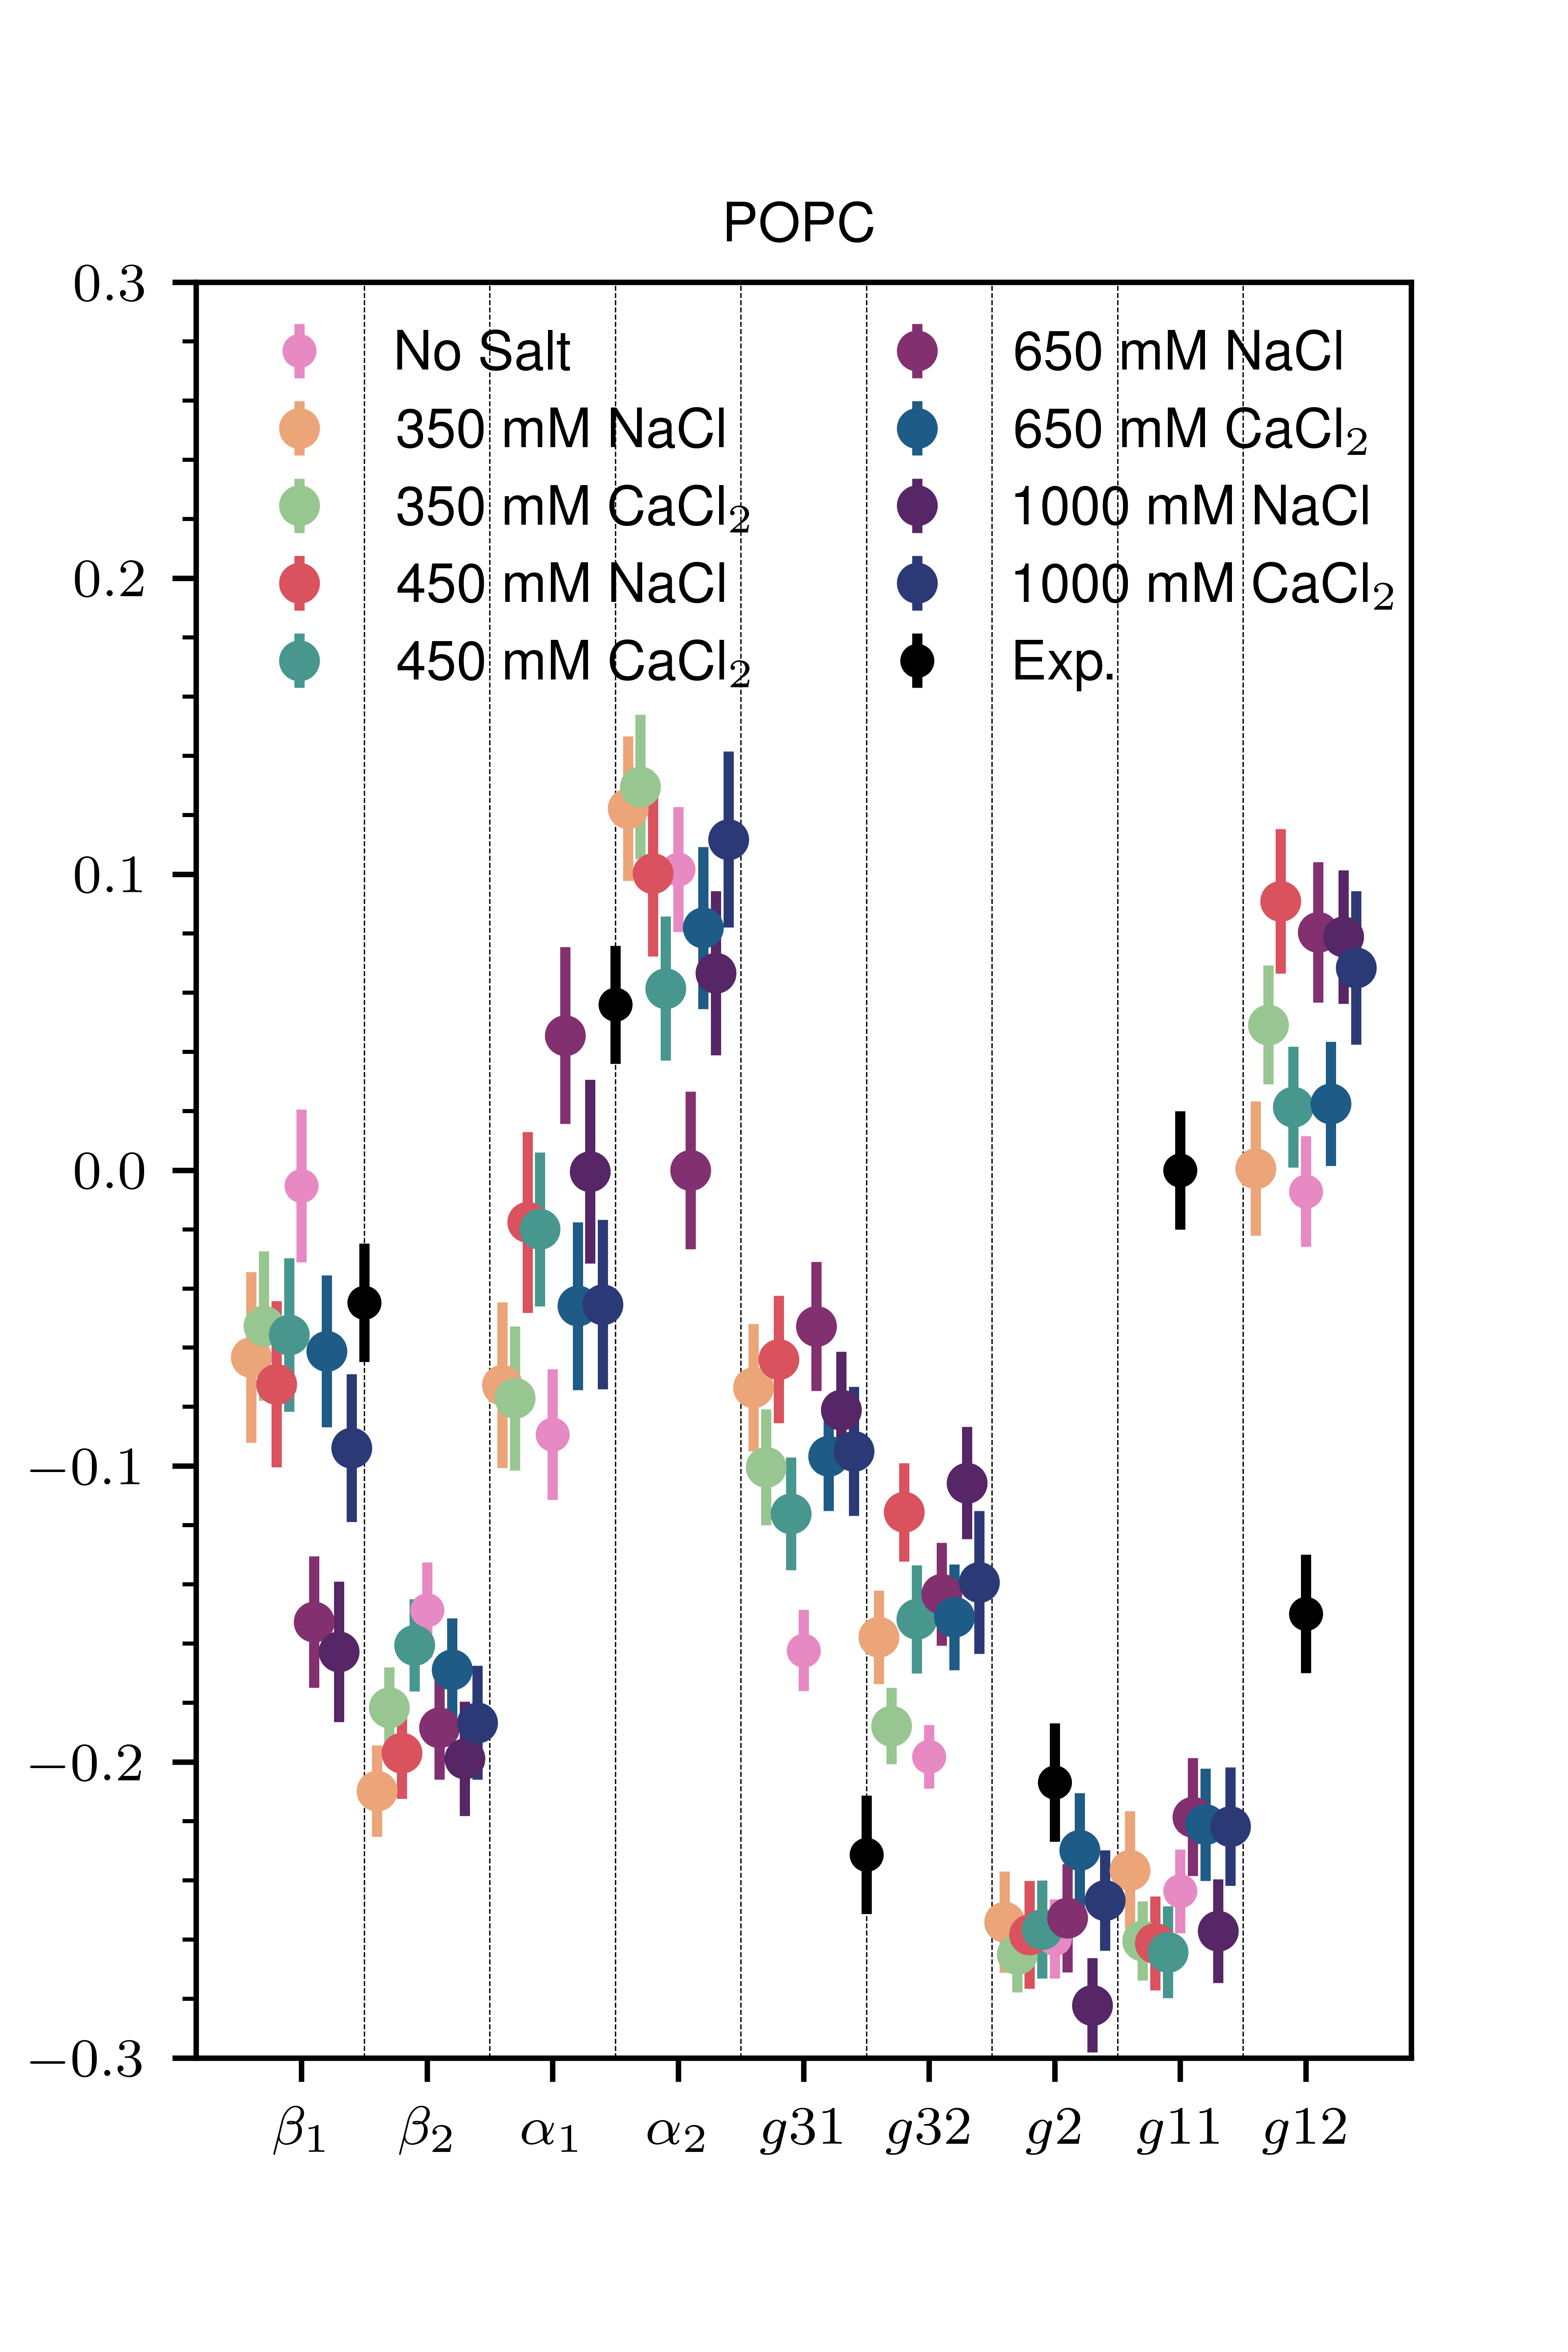
\includegraphics{popc_order_parameters_for_all.png}
	\caption{The head group and glycerol backbone order parameters $S_{CH}$ for the POPC simulations. The experimental values on the dashed lines mean that the different isomers 1/2 experimentally could not be resolved.}
	\label{fig:popc_order}
\end{figure}

\begin{figure}[!hbt]
	\centering
	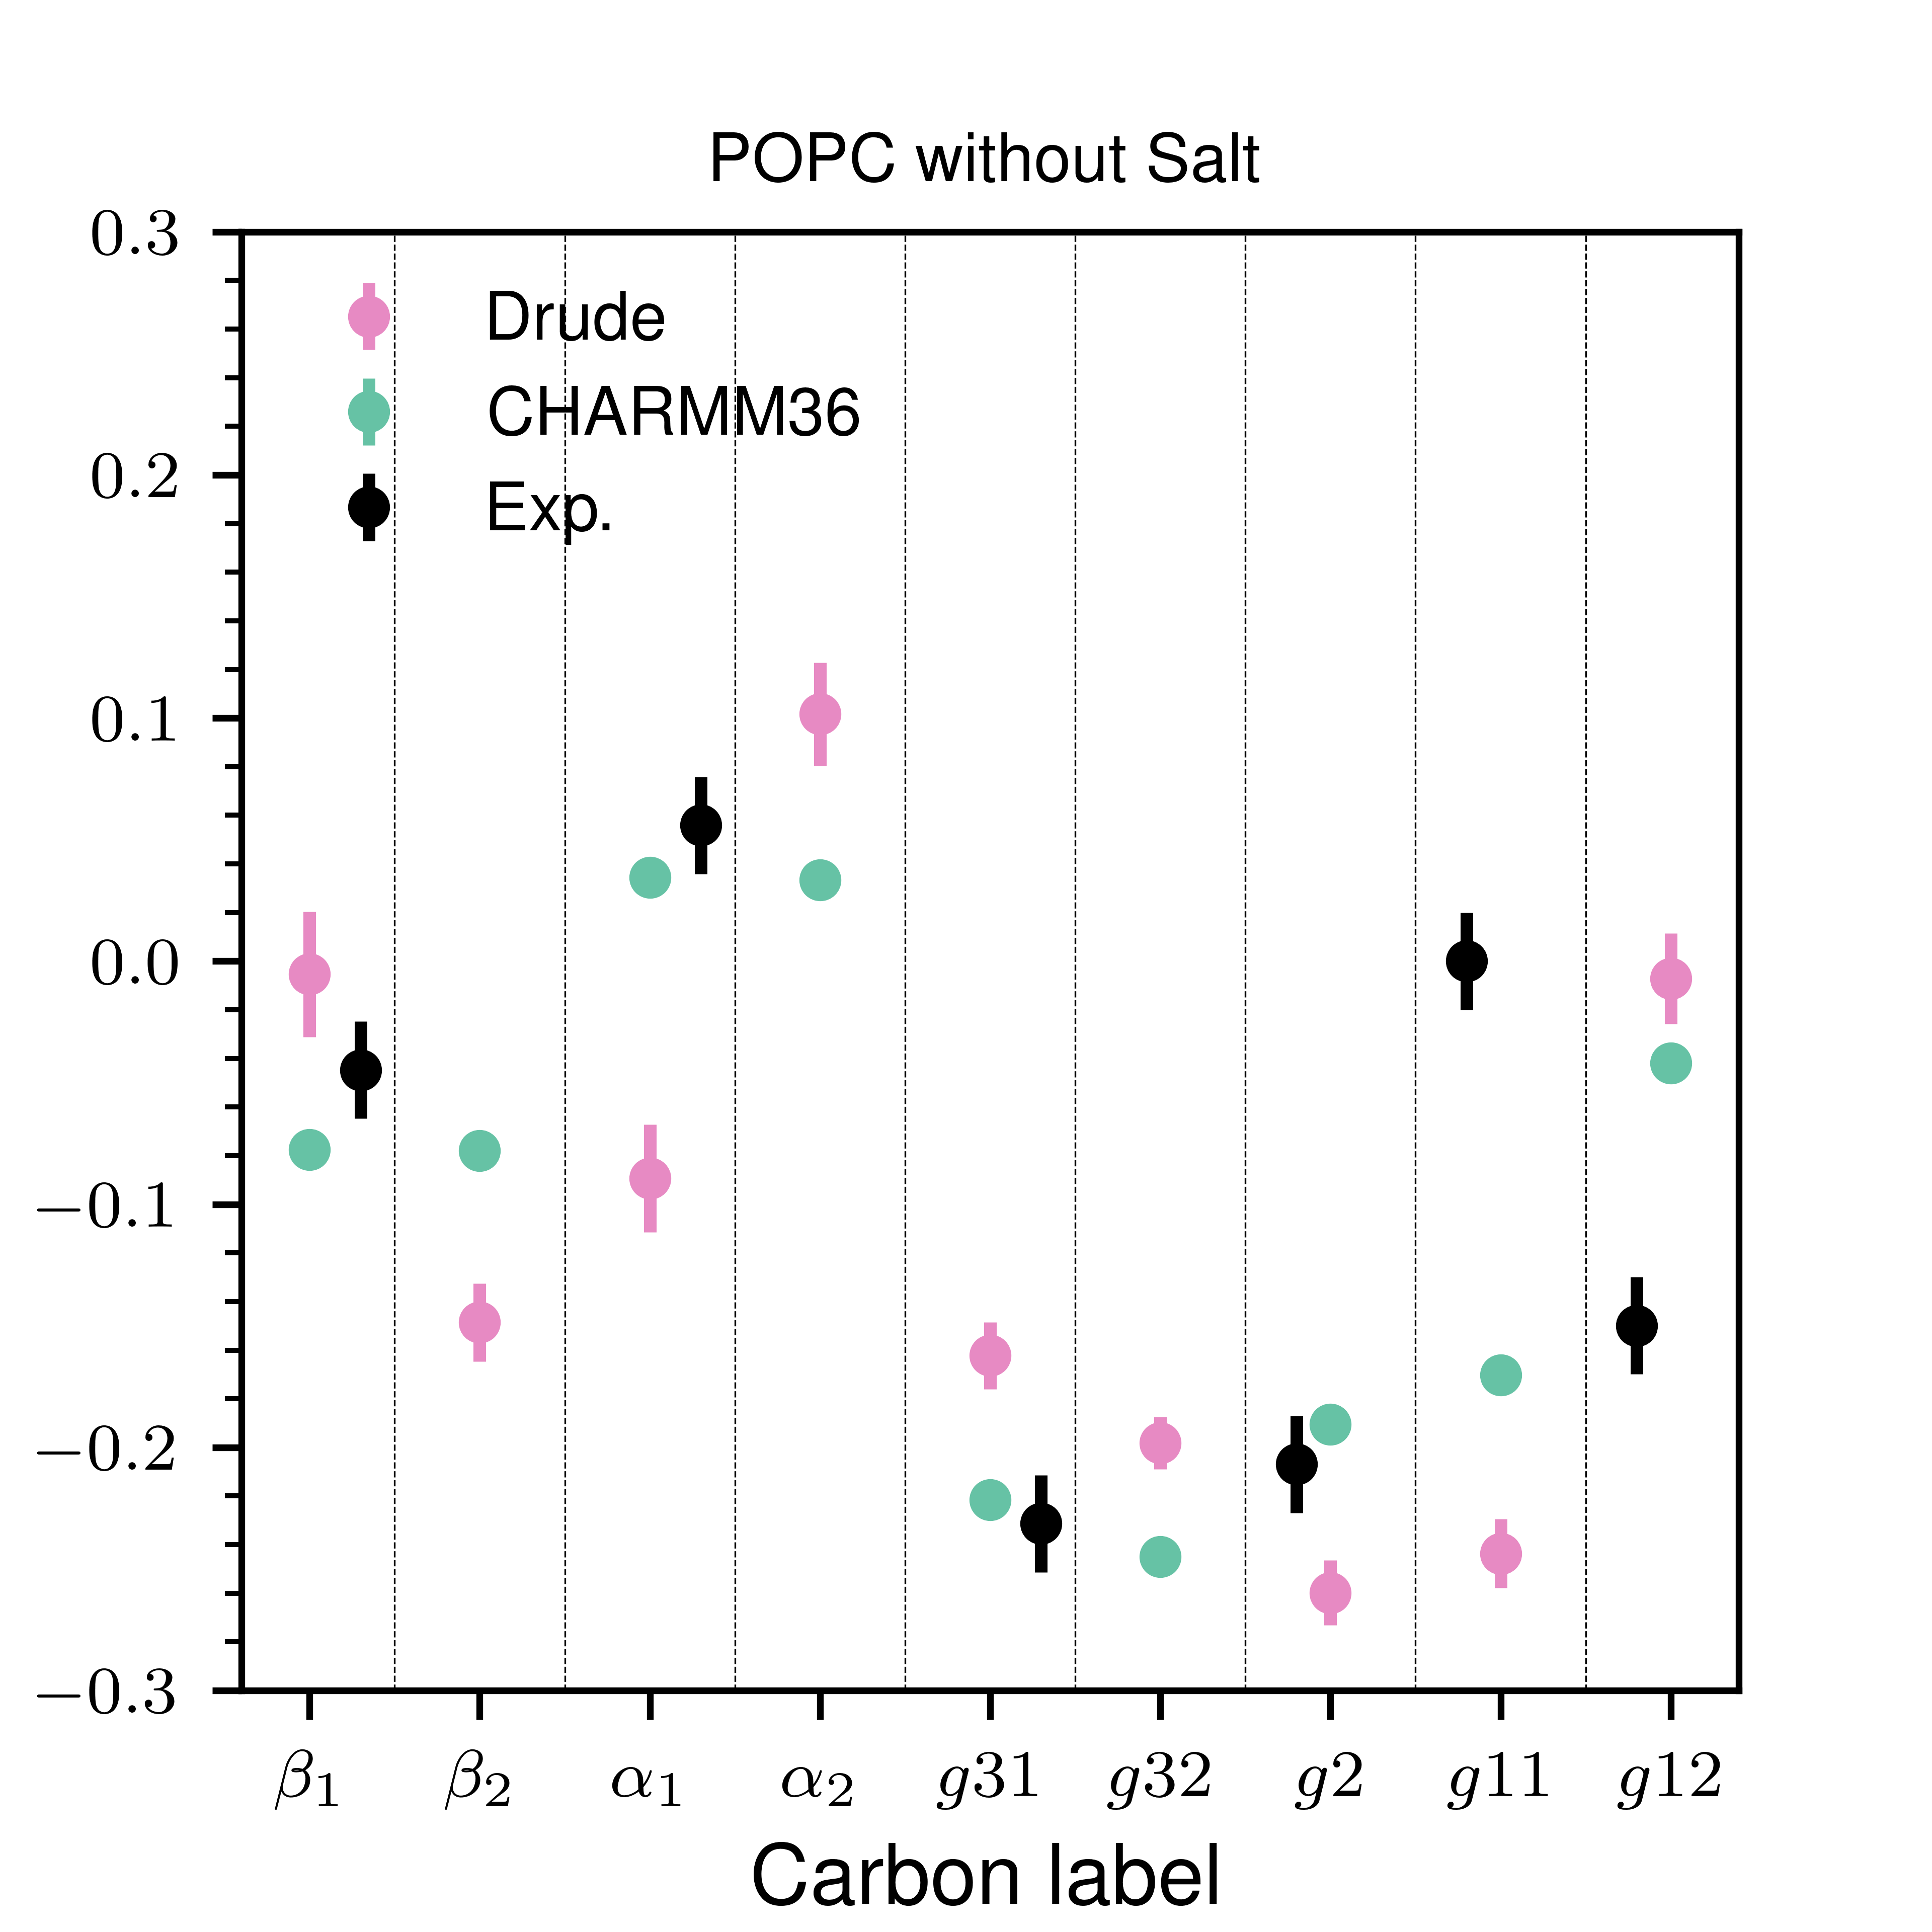
\includegraphics{popc_order_parameters_nosalt.png}
	\caption{The head group and glycerol backbone order parameters $S_{CH}$ for the POPC simulations without salt.}
	\label{fig:popc_order_no_salt}
\end{figure}

\begin{figure}[!hbt]
	\centering
	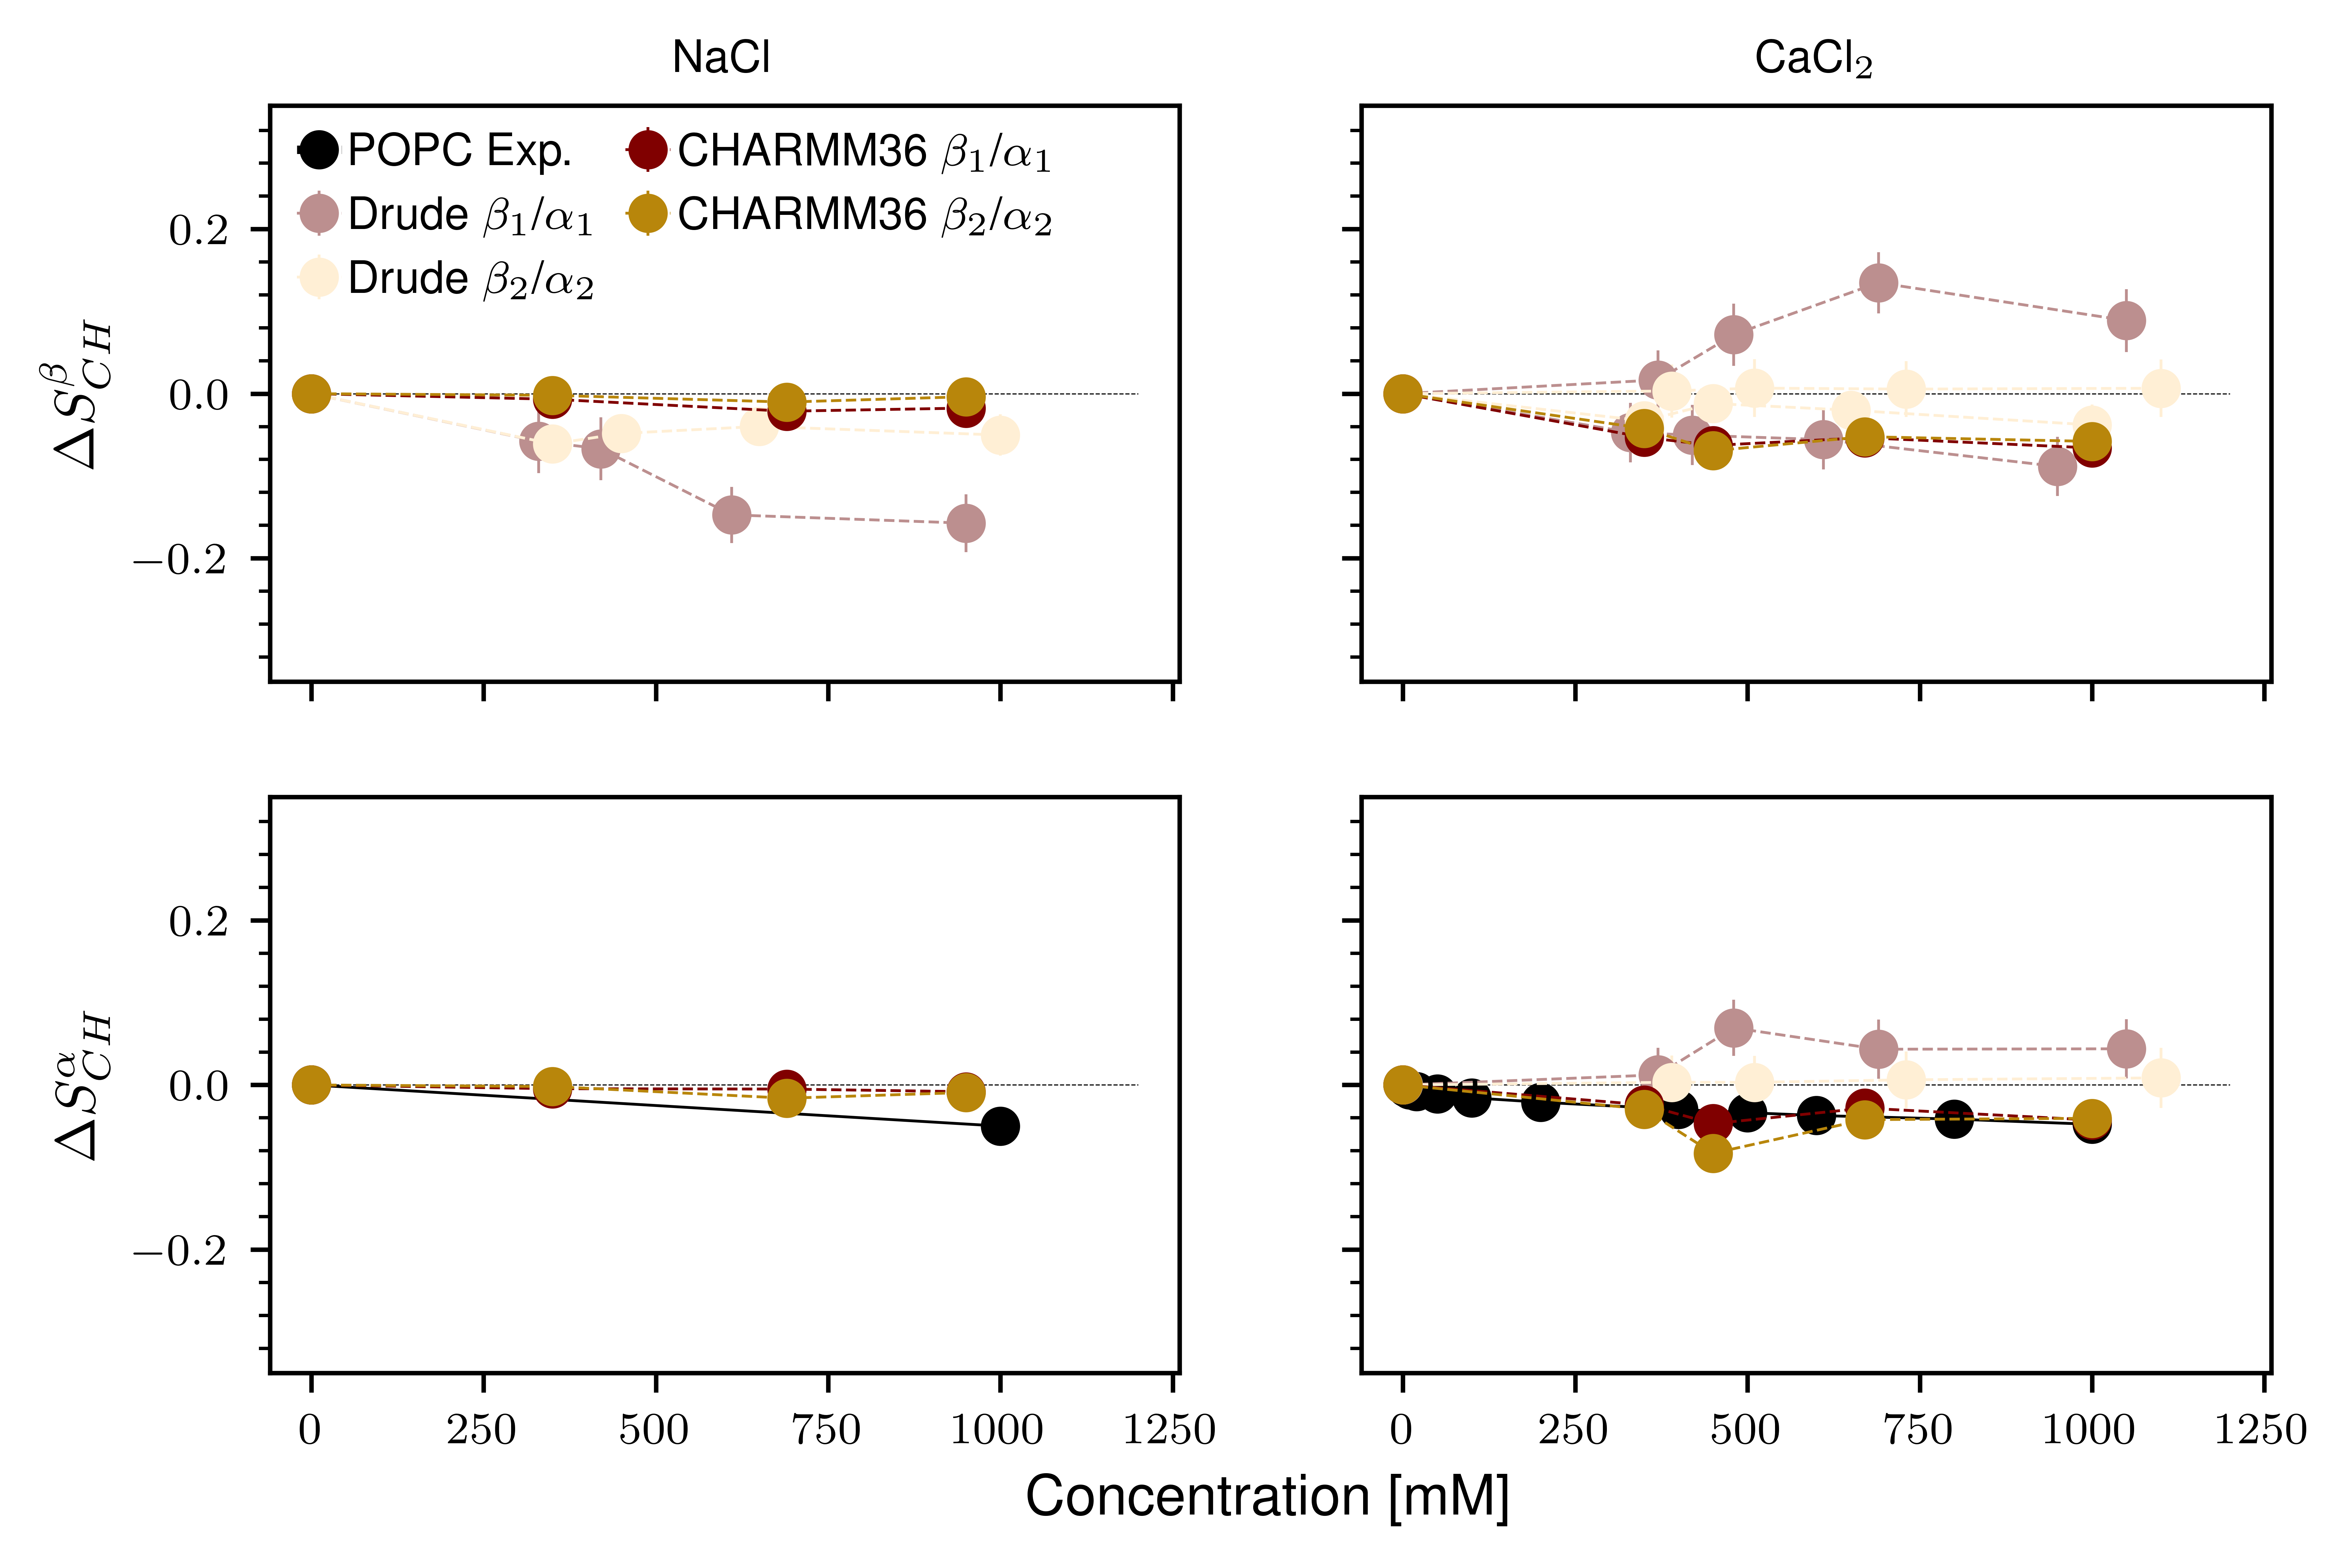
\includegraphics{popc_order_parameter_change.png}
	\caption{The change in the head group order parameters with respect to the simulations without salt as a function of the salt concentration.}
	\label{fig:popc_order_parameter_change}
\end{figure}

\begin{figure}[!hbt]
	\centering
	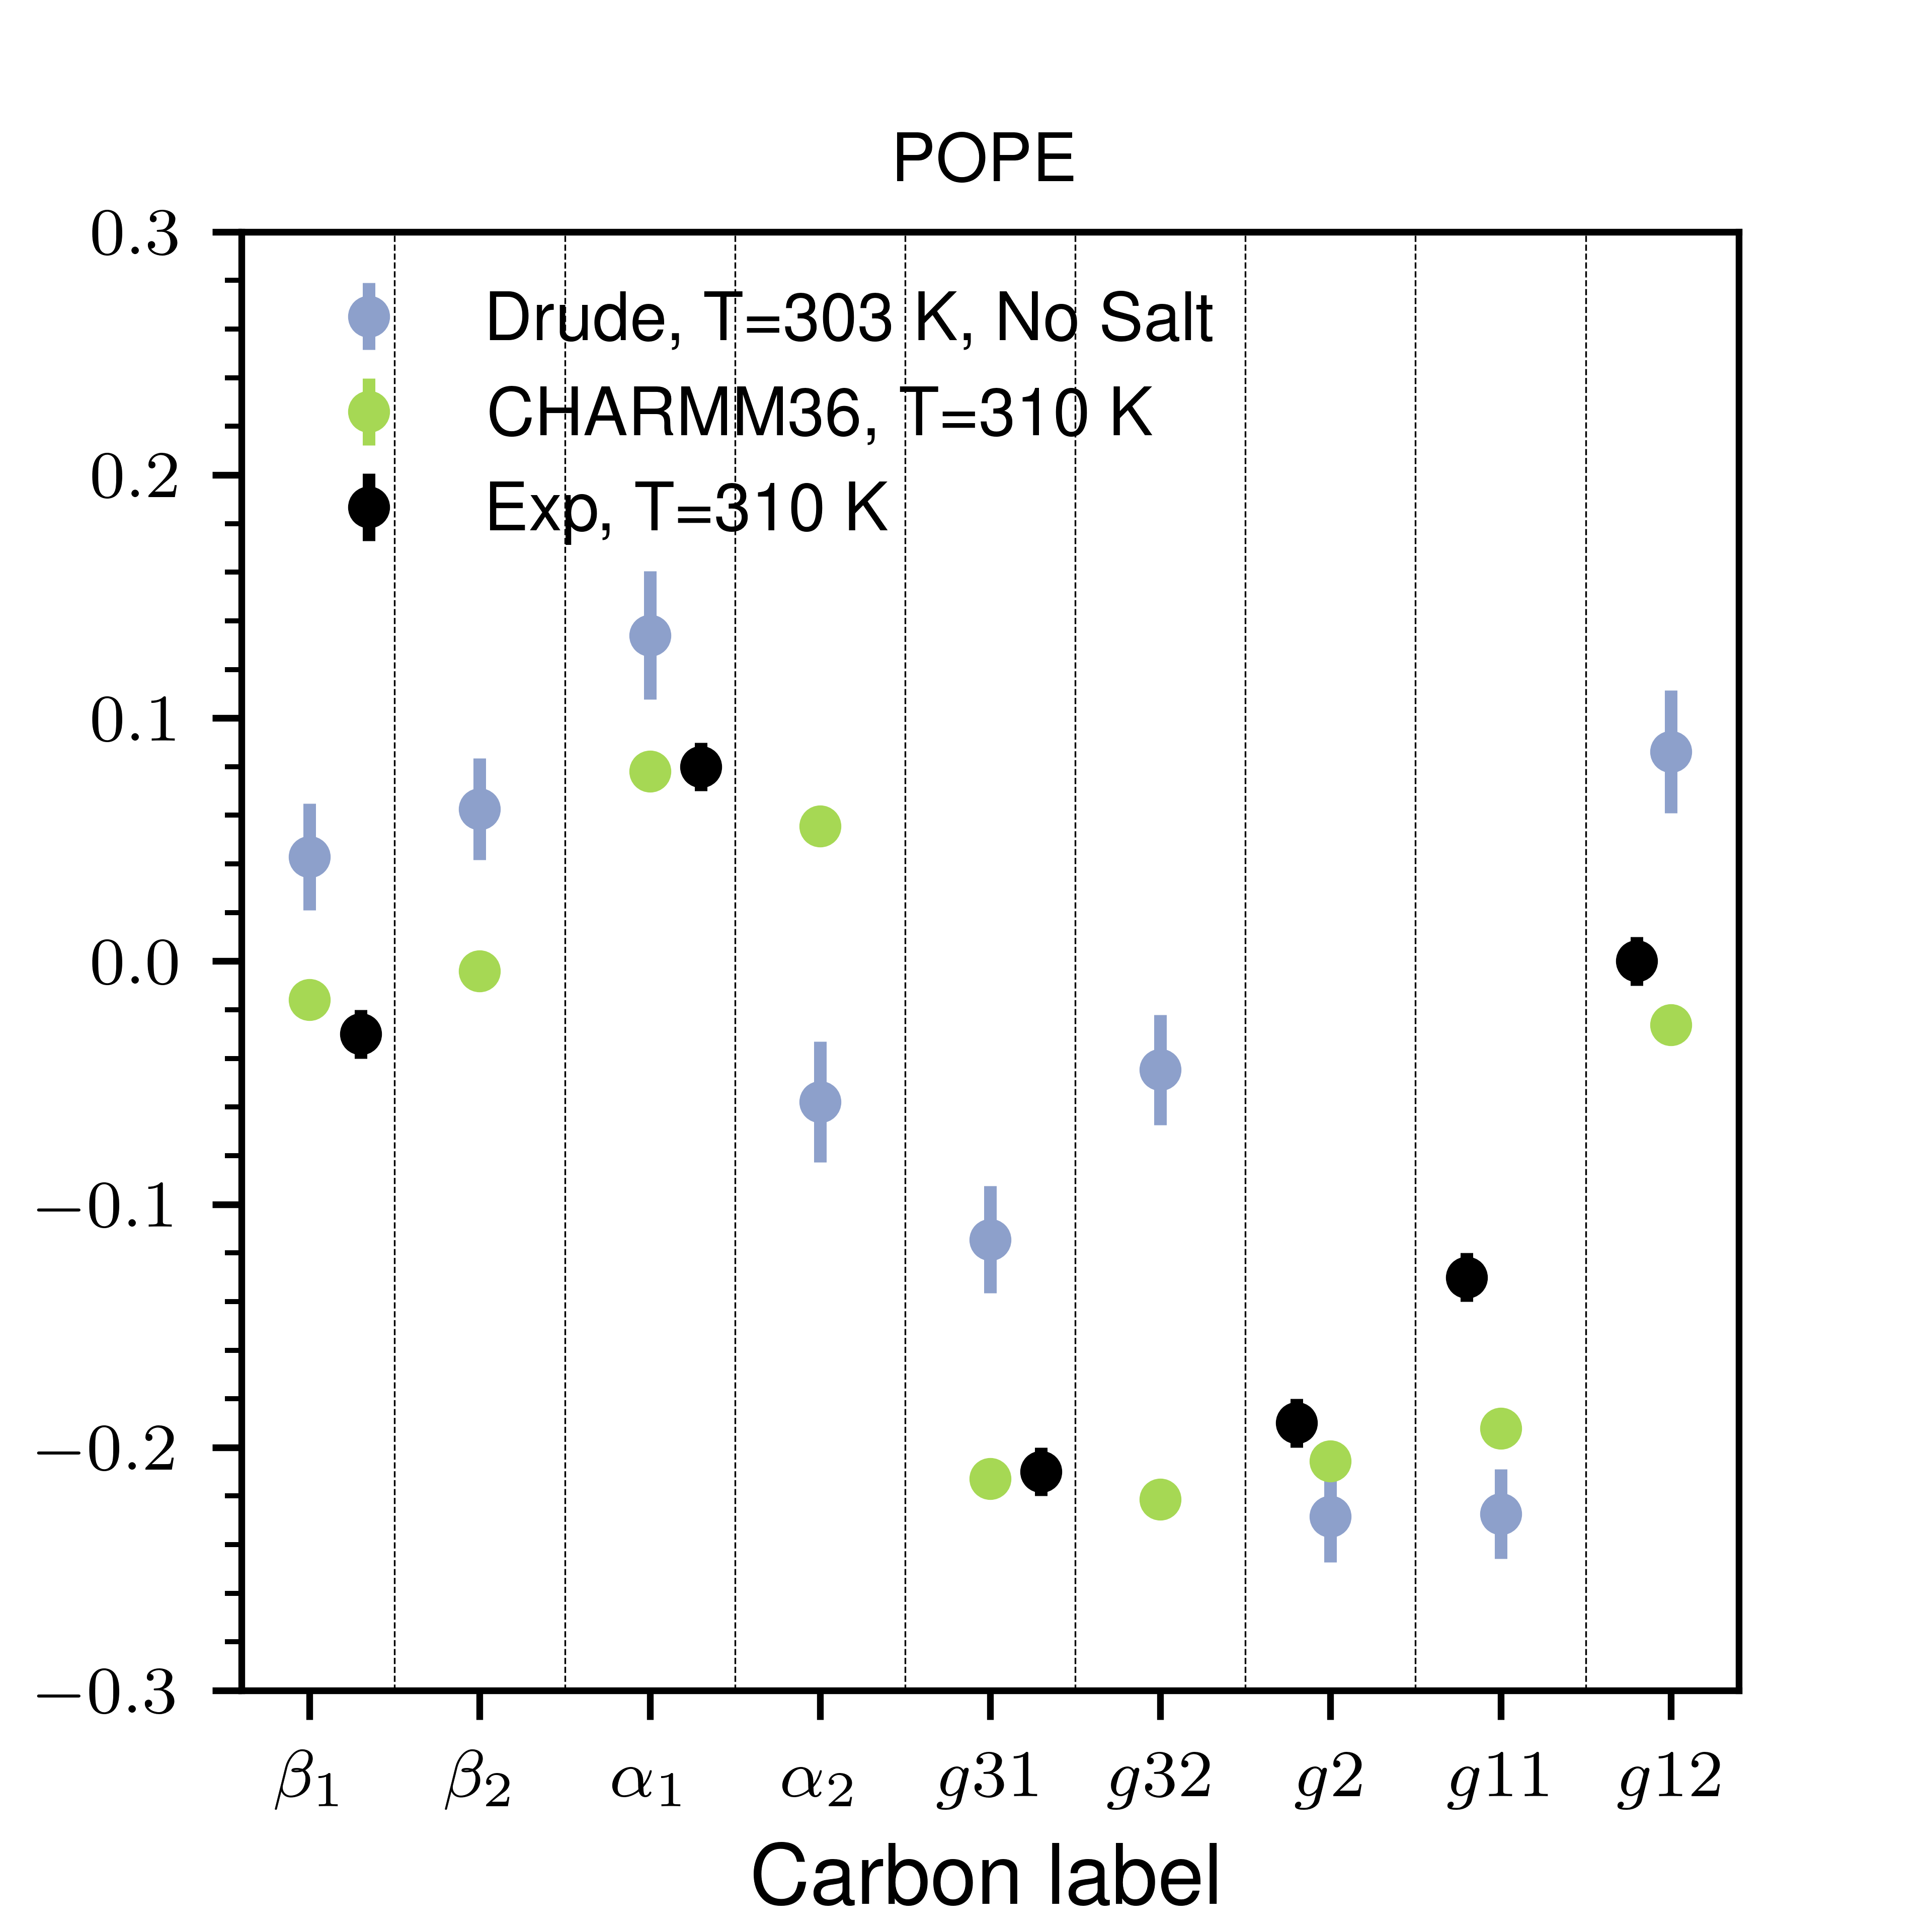
\includegraphics{pope_order_parameters.png}
	\caption{The head group and glycerol backbone order parameters $S_{CH}$ for the POPE simulations.}
	\label{fig:pope_order}
\end{figure}

\begin{figure}[!hbt]
	\centering
	\includegraphics{dihedral_distributions_for_all.png}
	\caption{The distributions of the torsion angles for the head group atoms}
	\label{fig:dihedral}
\end{figure}

\begin{figure}[!hbt]
	\centering
	\includegraphics{dihedral_distributions_no_salt.png}
	\caption{The distributions of the torsion angles for the head group atoms without the presence of salt.}
	\label{fig:dihedral_no_salt}
\end{figure}

\begin{figure}[!hbt]
	\centering
	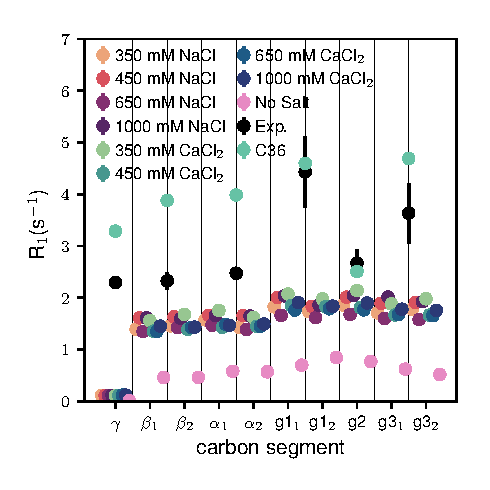
\includegraphics{correlation_times.eps}
	\caption{R1 times calculated for the POPC system. Experimental values are obtained from Ref.~\cite{antila2020quasi}}
	\label{fig:correlation_times}
\end{figure}

\clearpage

%%%%%%%%%%%%%%%%%%%%%%%%%%%%%%%%%%%%%%%%%%%%%%%%%%%%%%%%%%%%%%%%%%%%%
%% The "Acknowledgement" section can be given in all manuscript
%% classes.  This should be given within the "acknowledgement"
%% environment, which will make the correct section or running title.
%%%%%%%%%%%%%%%%%%%%%%%%%%%%%%%%%%%%%%%%%%%%%%%%%%%%%%%%%%%%%%%%%%%%%
\begin{acknowledgement}


\end{acknowledgement}

%%%%%%%%%%%%%%%%%%%%%%%%%%%%%%%%%%%%%%%%%%%%%%%%%%%%%%%%%%%%%%%%%%%%%
%% The same is true for Supporting Information, which should use the
%% suppinfo environment.
%%%%%%%%%%%%%%%%%%%%%%%%%%%%%%%%%%%%%%%%%%%%%%%%%%%%%%%%%%%%%%%%%%%%%
\begin{suppinfo}
\end{suppinfo}

%%%%%%%%%%%%%%%%%%%%%%%%%%%%%%%%%%%%%%%%%%%%%%%%%%%%%%%%%%%%%%%%%%%%%
%% The appropriate \bibliography command should be placed here.
%% Notice that the class file automatically sets \bibliographystyle
%% and also names the section correctly.
%%%%%%%%%%%%%%%%%%%%%%%%%%%%%%%%%%%%%%%%%%%%%%%%%%%%%%%%%%%%%%%%%%%%%
\bibliography{nmrlipidsPOL.bib}

\end{document}
